% !TEX root = ../Thesis.tex
\myChapter{Computed Tomography}\label{ch:ct}
\begin{flushright}{\slshape    
		So Long, and Thanks for All the Fish!} \\ \medskip
    --- \defcitealias{Adams1984}{Douglas Adams}\citetalias{Adams1984} \citep{Adams1984}
\end{flushright}
\bigskip
Computed tomography (\acs{cs}) is an imaging method where a three-dimensional image of the internal structure of an object is generated from a large series of two-dimensional x-ray images---single radiographies---which have been taken at equidistant angles
around a single rotation axis. The word tomography is derived from the greek words for tomos (\greektext tomos\latintext, slice) and grafia (\greektext graf'ia\latintext, describing).

\section{History}
Computed Tomography has come a long way since its commercial availability in the late 1970, where Sir Godfrey Hounsfield invented the first commercially available thanks to the upcoming availability of microcomputers.

The basic idea of todays tomography was already described in a patent granted to \citet{Frank1942} in the 1940s and several experiments around 1960--1965 showed the feasibility of three-dimensional reconstruction of an object which has been penetrated by radiation~\cite{Hsieh2003}. The first tomographic imagers produced radiographic images of selected sections of tissue by moving the x-ray source and the film over and under the patient in the opposite direction. This approach blurred structures lying under and over the selected region of interest. But this advance over conventional radiographies was insufficient to make two-dimensional tomographic images a useful diagnostic tool~\cite{Robb2003}.

While observing the planning of radiotherapy treatments, Allan M.\ Cormack realized that these treatments would greatly benefit if the x-ray attenuation coefficient distribution in the body would be known. In 1963 \citet{Cormack1963} reported about the investigation of a cylindrical disk with a diameter of \SI{20}{\centi\meter} which was made of two concentric aluminum cylinders embedded in an oak annulus. Using a collimated \isotope[60]{Co} source and a Geiger counter as a detector, \citeauthor{Cormack1963} was able to detect the absorption coefficients of the materials in the cylinder and repeated this experiments with an asymmetrical phantom consisting of aluminum and plastic. But since the calculations necessary for the extraction of the attenuation coefficients were both time-consuming and difficult, the presented results never really caught on. Cormack remarked that \begin{quote} There was virtually no response. The most interesting request for a reprint came from a Swiss Centre for Avalanche Research\graffito{Sigi, this quote is especially for you!}. The method would work for deposits of snow on mountains if one could get either the detector or the source into the mountain under the snow! \cite{Cormack1979}\end{quote}

In 1967, Godfrey N.\ Hounsfield started to develop the first clinical tomography scanners at the EMI Central Research Laboratories in the United Kingdom~\cite{Hsieh2003}. The first laboratory scanners took 9 days to acquire a scan of a slice of cow brain~\cite{Hounsfield1976}, but paved the path to the first clinically available \ac{ct} machines in hospitals and the scientific community. In 1979 Cormack and Hounsfield shared the Nobel Prize for Physiology and Medicine for their pioneering work in computed tomography.

From the early 1980s on, \ac{ct} imaging became an important tool to answer scientific questions both in medical and industrial applications.

Nonetheless these medical \ac{ct} scanners are in widespread use, their images suffer from relatively low spatial resolution in the sub-micrometer scale, which is often not enough to detect the finest details in biological samples. Since the radiation dose limitations imposed for medical scans often do not apply for biological samples which are dried, frozen or embedded in paraffin or plastic, more intense and collimated x-ray sources can be used. Using such sources in \ac{uct} stations enables to reach resolutions in the submicron range\todo{Citation?}. The use of synchrotron radiation as an x-ray source to produce highly intensive beams for microtomography was first proposed by \citet{Grodzins1983,Grodzins1983a}.

\section{Computed tomography principles}
To be able to introduce the physical principles of \ac{ct}, some important interactions of x-rays with matter have to be introduced. The energy of the x-ray photons in avalable at \ac{tomcat}, where all the experiments of this work have been performed is in the range of 6--\SI{45}{\kilo\electronvolt}\graffito{The experiments presented in part~\ref{part:results} have been performed between \SI{11.5}{\kilo\electronvolt} and \SI{12.6}{\kilo\electronvolt}.%
% XRM 11.5 keV
% Tsuda 12.398 keV
% Haberthuer 12.6 keV
}, we can thus limit the explanation to absorption, Rayleigh and Compton scattering. We neglect the description of electron-positron pair production, which occurs only for x-ray energies above \SI{1}{\mega\electronvolt}.

\subsection{Absorption}\label{sec:absorption}
In the relevant apsorption process---the so-called photoelectric effect---an incoming x-ray photon with energy $E_{\gamma}$ interacts with a bound atomic electron in a deep shell and is completely absorbed. This process only happens if $E_{\gamma}$ is greater than the binding energy $E_{Shell}$ of the shell electron and releases a photo-electron with the energy $\Delta E=E_{\gamma}-E_{Shell}$. This liberation creates a hole in the deep shell, which is immediately filled by electrons from outer shells of the atom. Since the electron from the outer shell is at a higher energy state than the inner shell electron, a cascade process is initated which results in the emision of radiation which is characteristic depending on the absorbing atom.

\subsection{Scattering}
\subsubsection{Compton scattering}
\citet{Compton1923} first described this inelastic scattering\graffito{In inelastic scattering the kinetic energy of an incident particle is not conserved.} effect which is observed when an incident photon with an Energy $E=h\nu$ transfers parts of its energy to a scattering electron which is then ejected from the atom. 

To conserve the overall momentum of the system, the electron recoils at an angle $\theta$ and the photon is scattered in a direction $\phi$ with a reduced energy $E=h\nu'$. If the photon still has enough energy left, the process may be repeated, if the photon is of lower energy, it can subsequently be absorbed as described above in section~\ref{sec:absorption}.

The energy of the recoiled electron is $\Delta E=h(\nu-\nu')$, where $h\nu'$ is given by equation~\ref{eq:hnu}
\begin{equation}
	h\nu'=\frac{h\nu}{1+\frac{h\nu}{m_{e}c^{2}}(1-cos\theta)}
	\label{eq:hnu}
\end{equation}\todo[inline]{or use $\lambda' - \lambda = \frac{h}{m_e c}(1-\cos{\theta})$ as in \url{http://is.gd/b9wj1}?}

\subsubsection{Coherent scattering}\todo{MOAR!}


\def\width{0.8\linewidth}%
\def\height{0.4944\linewidth}% =0.8*0.618
\begin{figure}
	\centering%
	% !TEX root = ../Thesis.tex
%\documentclass{article}
%\usepackage{tikz,pgfplots,siunitx}
%\usepackage[graphics,tightpage,active]{preview}
%\PreviewEnvironment{tikzpicture}
%\begin{document}
%%%%%%%%%%%%%%%%%%%%%%%%%%%%%%%%%%%%%%%%%%%%%%%%%%%%%%%%%%%%%%
%\pgfplotstableread{plotdata/InteractionPercentage-big.txt}\table
\pgfplotstableread{Plots/plotdata/InteractionPercentage-big.txt}\table
\pgfplotsset{
	legend style={
 		%at={(1.02,0.5)}, anchor=west,%left
 		at={(0.5,-0.2)}, anchor=north,%bottom
		cells={anchor=west},
		%font=\footnotesize,
		},
	xlabel=Photon Energy [\kilo\electronvolt],%
	ylabel=[\percent]
	}
\begin{tikzpicture}
	\begin{semilogxaxis}[%
		width=\width,%
		height=\height,%
		scale only axis,%
		no markers,
		xmin=0,%
		xmax=1e5,%
		ymin=0,%
		ymax=100,%
		grid=both%
		]
		\addplot [red, thick]
			table [x=keV, y=IntCoherent] from \table;
		\addplot [blue, thick]
			table [x=keV, y=IntCompton] from \table;
		\addplot [green, thick]
			table [x=keV, y=IntPhoto] from \table;
		\addplot [cyan, thick]
			table [x=keV, y=IntPair] from \table;
		\addplot [fill=lightgray, semitransparent]
			coordinates
			{(6,0) (6,100) (45,100) (45,0)}; 
		\legend{%
			Coherent (Rayleigh) scattering,%
			Incoherend (Compton) scattering,%
			Photoelectric absorption,%
			Pair production%
			}
	\end{semilogxaxis}
\end{tikzpicture}%
%%%%%%%%%%%%%%%%%%%%%%%%%%%%%%%%%%%%%%%%%%%%%%%%%%%%%%%%%%%%%%
%\end{document}%
	\caption[Interaction types]{Percentage of the different interaction types specified above as a function of the beam energy in water. The grey marked region is the approximate energy-range relevant for this work. Data from~\cite[Table 5-5]{Johns1983}.}%
	\label{fig:InteractionPercentage}%
\end{figure}

\begin{figure}
	\centering%
	% !TEX root = ../Thesis.tex
%\documentclass{article}
%\usepackage{tikz,pgfplots,siunitx}
%\usepackage[graphics,tightpage,active]{preview}
%\PreviewEnvironment{tikzpicture}
%\begin{document}
%%%%%%%%%%%%%%%%%%%%%%%%%%%%%%%%%%%%%%%%%%%%%%%%%%%%%%%%%%%%%%
%\pgfplotstableread{plotdata/InteractionPercentage-small.txt}\table
\pgfplotstableread{Plots/plotdata/InteractionPercentage-small.txt}\table
\pgfplotsset{
	legend style={
 		%at={(1.02,0.5)}, anchor=west,%left
 		at={(0.5,-0.35)}, anchor=north,%bottom
		cells={anchor=west},
		%font=\footnotesize,
		},
	xlabel=Photon Energy [\kilo\electronvolt],%
	%ylabel=[\percent]
	}
\begin{tikzpicture}
	\begin{axis}[%
		width=\width,%
		height=\height,%
		scale only axis,%
		no markers,
		xmin=0,%
		xmax=60,%
		ymin=0,%
		ymax=100,%
		grid=both,%
		xtick={0,10,...,60},%
		]
		\addplot [fill=lightgray, semitransparent]
			coordinates
				{(6,0) (6,100) (45,100) (45,0)};
		\addplot [fill=darkgray, semitransparent]
			coordinates
				{(11,0) (11,100) (13,100) (13,0)}; 
		\addplot [red, thick]
			table [x=keV, y=IntCoherent] from \table;
		\addplot [blue, thick]
			table [x=keV, y=IntCompton] from \table;
		\addplot [green, thick]
			table [x=keV, y=IntPhoto] from \table;
		\addplot [cyan, thick]
			table [x=keV, y=IntPair] from \table;
		\legend{%
			,,%needed for not having marked regions in legend
			Coherent (Rayleigh) scattering,%
			Incoherend (Compton) scattering,%
			Photoelectric absorption,%
			Pair production%
			}
	\end{axis}
\end{tikzpicture}
%%%%%%%%%%%%%%%%%%%%%%%%%%%%%%%%%%%%%%%%%%%%%%%%%%%%%%%%%%%%%%
%\end{document}%
	\caption[Interaction types, Detail]{Detailed view of the percentage of the different interaction types specified above as a function of the beam energy in water. The grey region is the approximate energy-range relevant for this work. Data from~\cite[Table 5-5]{Johns1983}. Unfortunately, the data below \SI{10}{\kilo\electronvolt} is missing.}%
	\label{fig:InteractionPercentage}%
\end{figure}

\subsection{Attenuation}
The net effect of the three effects described above can be summarized with the total linear attenuation coefficient shown in equation~\ref{eq:linear attenuation} below. This equation expresses the attenuation of a monochromatic\graffito{Monochromatic light is light of a single wavelength or energy, though in practice it often refers to a narrow wavelength range} beam as it passes through a material. The attenuation in this material of uniform density and atomic number can be expressed by an exponential relationship%
\begin{equation}%
	I=I_{0}e^{-(\tau+\sigma_{C}+\sigma_{R})x}%
	\label{eq:linear attenuation}%
\end{equation}%
, where $I$ and $I_{0}$ are the incident and transmitted intensities of the x-rays and $x$ is the distance which the x-rays travel through the material. $\tau$, $\sigma_{C}$ and $\sigma_{R}$ are the attenuation coefficients of the photoelectric, incoherent (Compton) and coherent (Rayleigh) scattering interactions in the material, respectively. Equation~\ref{eq:linear attenuation} is often expressed as
\begin{equation}
	I/I_{0}=e^{-\mu x}
	\label{eq:beer-lambert}
\end{equation}%
the so-called Beer-Lambert law, where $\mu$ is the attenuation coefficient of the material, which is depending on the incident x-ray photon energy~\cite{Hsieh2003}. 

Figure~\ref{fig:yag attenuation} shows the composition of the attenuation coefficient for Cerium doped \ac{yag} (\cf{Y3Al5O12}), which is used as a material for converting the incident x-rays to visible light. This so-called scintillator is part of the microtomography station at \ac{tomcat} and is described in detail later in section~\ref{sec:tomcat}.

\begin{figure}[htb]
	\centering
	\documentclass{article}
\usepackage{tikz,pgfplots}
\usepackage[graphics,tightpage,active]{preview}
\PreviewEnvironment{tikzpicture}
\begin{document}
%%%%%%%%%%%%%%%%%%%%%%%%%%%%%%%%%%%%%%%%%%%%%%%%%%%%%%%%%%%%%%
\pgfplotsset{every axis legend/.append style={
	at={(1.02,0.5)},
	anchor=west},legend plot pos=right}
\begin{tikzpicture}
	\begin{loglogaxis}[no markers,xmajorgrids,xminorgrids,ymajorgrids]
		\addplot table [x=PhotonEnergy, y=ScatteringCoherent] {plotdata/yag.txt};
		\addplot table [x=PhotonEnergy, y=ScatteringIncoherent] {plotdata/yag.txt};
		\addplot table [x=PhotonEnergy, y=PhotoelectricAbsorption] {plotdata/yag.txt};
		\addplot table [x=PhotonEnergy, y=PairNuclear] {plotdata/yag.txt};
		\addplot table [x=PhotonEnergy, y=PairElectron] {plotdata/yag.txt};
		\addplot table [x=PhotonEnergy, y=TotalWithCoherent] {plotdata/yag.txt};
		\addplot table [x=PhotonEnergy, y=TotalWithoutCoherent] {plotdata/yag.txt};	
		\legend{ScatteringCoherent,%
			ScatteringIncoherent,%
			ScatteringIncoherent,%
			PhotoelectricAbsorption,%
			PairNuclear,%
			PairElectron,%
			TotalWithCoherent,%
			TotalWithoutCoherent}
	\end{loglogaxis}
\end{tikzpicture}
%%%%%%%%%%%%%%%%%%%%%%%%%%%%%%%%%%%%%%%%%%%%%%%%%%%%%%%%%%%%%%
\end{document}
	\caption[Total attenuation coefficient of Ce:YAG]{Total attenuation coefficient of Ce:YAG (\cf{Y3Al5O12}), the scintillator material used for converting the incident x-rays to visible light in chapters~\ref{ch:xrm2008}--\ref{ch:haberthuer2010}. Note that pair production starts for energies above \SI{1}{\mega\electronvolt} and can thus be safely ignored for the energy-ranges in this work. Data obtained from the photon cross section database~\cite{XCOM}.}
	\label{fig:yag attenuation}
\end{figure}

\subsection{Sampling Theorem}
\subsection{Reconstruction (FBP, gridrec)}

In general, \ac{ct} refers to the cross-sectional imaging of a sample from transmission images or projections recorded at several angular positions around the sample~\cite{Kak2002}.

In medical \ac{CT}-scanners, the transmission images are generally obtained while the radiation source and the detector rotate around the body part to be imaged. In micro-computed and synchrotron based tomography, the source and detector are fixed, while the sample to be imaged rotates around a chosen axis. During the imaging process multiple transmission images -- essentially single radiographic images -- are obtained at several angles over a \unit{180}{\degree} or \unit{360}{\degree} rotation. Before and after the scan, so-called dark and flat images (FI) are recorded. The dark images record the camera noise and dark current, while the flat images record the beam profile. After baseline correction of the projections (PI) the average of the dark images is subtracted. The projections are then normalized to the flat images as seen in equation~\ref{eq:cpr}, resulting in so-called corrected projections (CPR).

\begin{equation}
	CPR=-ln\left(\frac{PI}{FI}\right)=ln(FI)-ln(PI)
	\label{eq:cpr}
\end{equation}

The corrected projections are then transformed into so-called sinograms, where the $n$\textsuperscript{th} sinogram is composed of the $n$\textsuperscript{th} line of each projection.

The sinograms inherit their name because the Radon transformation\graffito{The Radon transformation was described in 1917 by Johann~\citet{Radon1917} and is the mathematical basis for tomographic imaging.} of a Dirac delta peak resembles a sine wave. The Radon transformation of a cluster of objects appears as an overlay of blurred sine waves with different amplitudes and phases.

One sinogram contains the information of one plane or slice of the reconstructed tomographic image. We can thus reconstruct the $n$\textsuperscript{th} slice of the tomographic data-set from the $n$\textsuperscript{th} sinogram using different reconstructing algorithms, e.g.\ a standard filtered back-projection algorithm. In a reconstructed slice, the absorption properties of the sample at a certain height are encoded by the gray values of the image.

\begin{figure}
	\missingfigure{Sinogram?}
	\caption{Sinogram}
	\label{fig:sinogram}
\end{figure}

\section{Synchrotron Radiation}
Synchrotron facilities use the fact that a accelerated particles travelling on a curved trajectory emit radiation. If charged particles at relativistic speed are undergo a change of direction (\ie in a magnetic field) so-called synchrotron radiation is emitted. 

Synchrotron radiation was first observed as energy loss in electron storage rings used for high energy physics experiments. First sources for scientific use were beamports at such facilities, which utilized otherwise lost radiation. Dedicated second-generation synchrotron radiation sources have been built over the years; these were ring-like structures using a series of magnets to control the accelerated particles. Current---third-generation---synchrotron radiation facilities are composed of many straight sections of different lengths, specially optimized to accommodate different magnetic structures used to generate the synchrotron radiation~\cite{Stampanoni2002a,Margaritondo2002,wwwsls}. 

\subsection{Bending Magnets, Undulators and Wigglers}
The three magnetic structures used in synchrotron facilities are bending magnets, undulators and wigglers. All three emit radiation with different characteristics and intensities.

Bending Magnets are used to create a homogeneous magnetic field over a defined distance. This forces accelerated particles injected into the bending magnet to travel on a circular trajectory. The result is a fan of radiation in the tangential direction of the bend\graffito{Such magnets are also used in traditional televisions, which contain a cathode ray tube, which is essentially a small particle accelerator. They move the electron beam over the screen of the TV tube in a controlled way.~\cite{wiki:dipolemagnet}}.

\begin{figure}[htb]
	\centering
	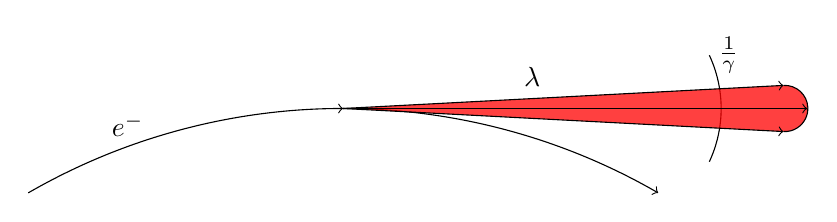
\begin{tikzpicture}[scale=0.8]
		\def\alpha{3}
		\def\length{7}
		% arc
			\draw [<-] (0,0) arc (90:110:10) node [above] {$e^-$} arc (110:120:10);
			\draw [->] (0,0) arc (90:60:10);
		% beam angle
			\draw (\length-1,0) arc (0:-25:2);
			\draw (\length-1,0) arc (0:25:2) node [right] {$\frac{1}{\gamma}$};
		% beam
			\def\arclength{0.36685445498128842827164077131789} % arclength = tan(\alpha)*\length
			\fill [color=red,nearly opaque] (0,0) -- (\alpha:\length) arc (90+\alpha:-90-\alpha:\arclength) -- cycle; 
			\draw (\alpha:\length) arc (90+\alpha:-90-\alpha:\arclength);
			\node at (3,.5) {$\lambda$};
		% arrows
			\draw [->] (0,0) -- (\alpha:\length);
			\draw [->] (0,0) -- (\length+\arclength,0);
			\draw [->] (0,0) -- (-\alpha:\length);
	\end{tikzpicture}
	\caption[Bending magnet radiation]{Bending magnet radiation of wavelength $\lambda$ produced by a relativistic electron in an uniform magnetic field. The emission angle is typically $\frac{1}{\gamma}$ where $\gamma$ is the Lorentz contraction factor. Adapted from~\cite{Attwood2007}.}
	\label{fig:bending magnets}
\end{figure}

Undulators consist of periodic structures of dipole magnets with relatively weak fields. The the alternating static magnetic field forces the electrons to harmonically oscillate as they move in the axial direction, resulting in an undulating motion of the particles in the structure. The weak magnetic fields cause small amplitude undulation which leads to a narrow radiation cone as a result. Through coherent addition of the tightly confined electron beam, the produced radiation is emitted with small angular divergence and concentrated in narrow energy bands~\cite{Stampanoni2002a}.

Wigglers are the strong brothers of the undulators. Due to stronger magnetic fields the oscillation amplitude of the electrons and the emitted radiation power are larger and the radiation cone is broader.

The relativistic electrons are usually produced by a hot filament. They are then pre-accelerated and injected into the storage ring by a linear accelerator. Bending magnets along the storage ring keep the electrons on their circular path. Quadrupole magnets along the ring are used to improve the geometrical characteristics of the electron beam, \ie reduce the transverse section and angular spread of the beam, hence improving the so-called brightness of the source~\cite{Margaritondo2002}.

\section{The Swiss Light Source}
The \ac{sls} at the \ac{psi} in Villigen, Switzerland is a third-generation synchrotron light source. With an energy of \SI{2.4}{\giga\electronvolt}, it provides photon beams of high brightness for research in materials science, biology and chemistry.

\renewcommand{\imsize}{0.618\linewidth}%
\begin{figure}[htb]
	\centering
	\includegraphics[width=\imsize]{img/SLS_beamlines_2008}
	\caption[Beamlines at the Swiss Light Source]{Beamlines at the \ac{sls}. Image from the \href{http://sls.web.psi.ch/view.php/beamlines/}{SLS Website}}
	\label{fig:beamlines}
\end{figure}

\section{tomcat}\label{sec:tomcat}
At \acf{tomcat} the user can perform absorption as well as phase contrast imaging with an isotropic voxel size ranging from \SI{350}{\nano\meter} up to \SI{14.8}{\micro\meter} depending on the chosen magnification. Typical acquisition times are in the order of a few minutes for a full sample, depending on the selected energy and resolution. A detailed explanation of the beamline for \ac{tomcat}, where all the tomography data for this thesis has been presented by \citet{Stampanoni2006a}.

As a short rundown the most important features of the beamline are presented here: The \ac{tomcat} beamline is located at the X02DA port of the SLS and started regular user operation in June 2006. Synchrotron light is delivered by a \SI{2.9}{\tesla} superbend which is magnetic field approximately double the strength of the normal \ac{sls} bending magnets. This enables to have a high critical energy of the source (\SI{11.1}{\kilo\electronvolt}, corresponding to a wavelength of \SI{1.22}{\angstrom}) and results in a considerable increase of flux at for hard X-rays. A double crystal multilayer monochromator is the main optical component of the beamline an is used to select the energy of the beam incident on the sample (Energy range from 6--\SI{45}{\kilo\electronvolt}, with a bandwidth of a few percent down to a few permille).

Once inside the measuring hut, the beam is travelling through a pipe and collimated onto the sample. After penetration of the sample, the X-rays are converted to visible light by a so-called scintillator\graffito{The latin word \textit{scintillare} can be translated with sparkle or flicker.}. Charged particles excite the scintillator material and this excitation energy is then subsequently emitted by fluorescence photons at a longer wavelength, which enables the detection of the incident light with a \ac{ccd}-camera. The \ac{ccd}-camera at \ac{tomcat} features a detector with 2048$\times$2048 pixels with a size of 7.4$\times$\SI{7.4}{\micro\meter} each. Between the scintillator and the \ac{ccd}-sensor an interchangeable microscope objectives enable to choose a wide range of the pixel size, ranging from 350$\times$\SI{350}{\nano\meter\squared}\todo{What about the 40$\times$ magnification?} up to 5.6$\times$\SI{5.6}{\micro\meter}. The resulting field of view of a standard scan can thus easily be varied from 0.75$\times$\SI{0.75}{\milli\meter\squared} up to 11.45$\times$\SI{11.45}{\milli\meter\squared}\graffito{See chapter~\ref{ch:haberthuer2010} presenting a method for increasing the field of view of tomography endstations.}.

\renewcommand{\imsize}{0.5\linewidth}
\begin{figure}[htb]
	\subfloat[Overview of the TOMCAT end-station: The blue structure behind the control notebook is the sample stage with the sample holder on the rotation stage on top of it. The black structure above contains the scintillator, the microscope optics and the camera.]{%
		\includegraphics[width=\imsize]{img/TOMCAT1}%
		\label{subfig:TOMCAT1}%
		}%
	\subfloat[Detail of the microscope optics: The sample holder with a mounted standard electron microscopy sample table is carrying a small piece of a rat lung. The round structure behind the sample contains the different objectives. The square visible under the label on the objective revolver is the scintillator which is used to convert the x-ray beam into visible light, which after magnification is then recorded with the CCD-camera.]{%
		\includegraphics[width=\imsize]{img/TOMCAT2}%
		\label{subfig:TOMCAT2}%
		}%
	\caption{Images of the TOMCAT beamline.}
\end{figure}

The sample positioning in the beam and the scanning parameters are controlled from outside the measuring hut through an \ac{epics} by the national laboratory of \href{http://www.aps.anl.gov/epics/}{Argonne in the USA}. After the start of the scan sinograms (see chapter~\ref{ch:ct}) are calculated on the fly and the tomographic reconstruction can be initialised using a web-based interface. This interface and the general workflow has been described by \citet{Hintermueller2010}.

After the reconstruction of the tomographic datasets on a node computing cluster of five \SI{64}{\bit} Opteron machines with four cores and \SI{8}{\giga\byte} \acs{ram} each the resulting data can be transferred to the home laboratory immediately after the beam time shifts.